\hypertarget{results}{%
\section{Results}}

\hypertarget{timing-improves-the-six-primary-crps-contrasts}{%
\subsection{Timing improves the six primary CRPS contrasts}}

Table~\ref{tab:primary} and Figure~\ref{fig:primary} show lower mean CRPS with timing in all six comparisons. All adjusted intervals lie below zero. The effect magnitudes differ: relative reductions range from 0.69\% to 4.31\% on Weibo and from 7.25\% to 13.48\% on SEISMIC. The 0.69\% reduction for Weibo NGBoost is small in relative terms despite its interval excluding zero. Evidence of a nonzero average improvement and the size of that improvement should therefore be reported separately.


\begin{table*}[t]
\caption{Primary held-out information contrasts. Lower CRPS is better. Adjusted intervals use the six-comparison Bonferroni family.}\label{tab:primary}
\centering\footnotesize\setlength{\tabcolsep}{3pt}\renewcommand{\arraystretch}{1.17}
\begin{tabularx}{\textwidth}{>{\hsize=0.7000000000000001\hsize\linewidth=\hsize\raggedright\arraybackslash}X>{\hsize=0.7000000000000001\hsize\linewidth=\hsize\raggedright\arraybackslash}X>{\hsize=0.77\hsize\linewidth=\hsize\raggedright\arraybackslash}X>{\hsize=0.77\hsize\linewidth=\hsize\raggedright\arraybackslash}X>{\hsize=0.77\hsize\linewidth=\hsize\raggedright\arraybackslash}X>{\hsize=1.61\hsize\linewidth=\hsize\raggedright\arraybackslash}X>{\hsize=0.9800000000000001\hsize\linewidth=\hsize\raggedright\arraybackslash}X}
\toprule
\textbf{Source} & \textbf{Family} & \textbf{I0 CRPS} & \textbf{I1 CRPS} & \textbf{I1 - I0} & \textbf{Adjusted interval} & \textbf{Relative reduction} \\ \midrule
Weibo & Hurdle & 124.126 & 121.286 & -2.840 & {[}-4.945, -1.090{]} & 2.29\% \\
Weibo & QRF & 100.990 & 96.640 & -4.350 & {[}-7.578, -0.397{]} & 4.31\% \\
Weibo & NGBoost & 111.249 & 110.484 & -0.765 & {[}-1.394, -0.273{]} & 0.69\% \\
SEISMIC & Hurdle & 52.036 & 45.022 & -7.014 & {[}-10.134, -4.956{]} & 13.48\% \\
SEISMIC & QRF & 42.875 & 39.058 & -3.817 & {[}-4.826, -2.855{]} & 8.90\% \\
SEISMIC & NGBoost & 42.522 & 39.440 & -3.083 & {[}-4.107, -1.890{]} & 7.25\% \\
\bottomrule\end{tabularx}
\end{table*}


\begin{figure*}[t]\centering
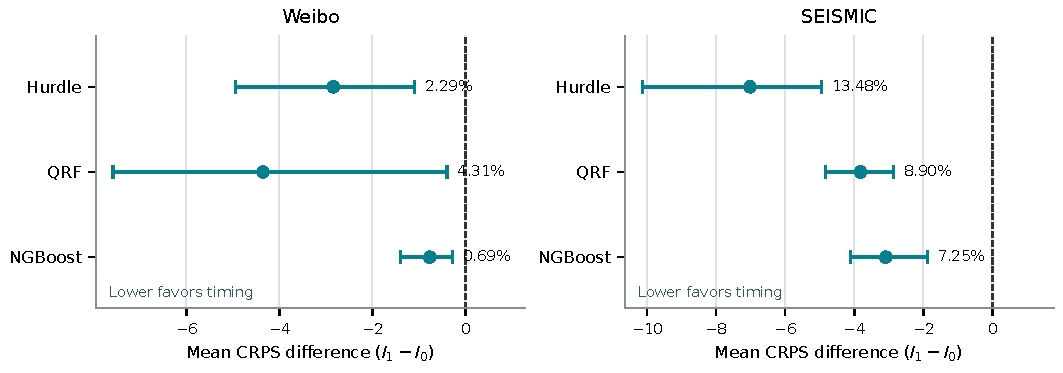
\includegraphics[width=\textwidth]{figures/primary_contrasts.pdf}
\caption{Mean CRPS changes from adding timing, with conditional adjusted intervals from 10,000 paired resamples per source. Labels give relative point reductions. Separate count scales are used; this is not a cross-source interaction test.}\label{fig:primary}
\end{figure*}

The per-window descriptive means favor \(I_1\) in all 18 primary-family/source/window combinations. However, Weibo NGBoost changes little at 15 minutes (113.285 to 113.222) and 60 minutes (89.374 to 89.085). Source and model differences persist beyond the aggregate result; no window-specific significance claim is made. Supplementary Section S4 provides every per-window value.

\hypertarget{conditional-empirical-forecasts-are-strong-references}{%
\subsection{Conditional empirical forecasts are strong references}}

Table~\ref{tab:all} places the information contrasts in a broader descriptive comparison. Conditioning the empirical distribution on prefix size reduces CRPS from 126.569 to 103.816 on Weibo and from 56.224 to 42.740 on SEISMIC. On SEISMIC this simple conditional reference lies close to the size-only QRF and NGBoost procedures. Timing-augmented QRF has the lowest mean CRPS among the evaluated procedures in both sources, at 96.640 and 39.058. The six primary intervals do not test QRF's superiority over other families.


\begin{table*}[t]
\caption{Mean test CRPS of all procedures. Cross-family rankings are descriptive; dashes denote undefined information sets.}\label{tab:all}
\centering\footnotesize\setlength{\tabcolsep}{3pt}\renewcommand{\arraystretch}{1.17}
\begin{tabularx}{\textwidth}{>{\hsize=1.6\hsize\linewidth=\hsize\raggedright\arraybackslash}X>{\hsize=0.8500000000000001\hsize\linewidth=\hsize\raggedright\arraybackslash}X>{\hsize=0.8500000000000001\hsize\linewidth=\hsize\raggedright\arraybackslash}X>{\hsize=0.8500000000000001\hsize\linewidth=\hsize\raggedright\arraybackslash}X>{\hsize=0.8500000000000001\hsize\linewidth=\hsize\raggedright\arraybackslash}X}
\toprule
\textbf{Procedure} & \textbf{Weibo I0} & \textbf{Weibo I1} & \textbf{SEISMIC I0} & \textbf{SEISMIC I1} \\ \midrule
Empirical by window & 126.569 & --- & 56.224 & --- \\
Conditional empirical & 103.816 & --- & 42.740 & --- \\
Poisson GLM & 148.384 & 146.924 & 66.422 & 59.117 \\
NB2 GLM & 123.562 & 120.559 & 52.041 & 45.554 \\
Hurdle & 124.126 & 121.286 & 52.036 & 45.022 \\
QRF & 100.990 & 96.640 & 42.875 & 39.058 \\
NGBoost & 111.249 & 110.484 & 42.522 & 39.440 \\
\bottomrule\end{tabularx}
\end{table*}


\begin{figure*}[t]\centering
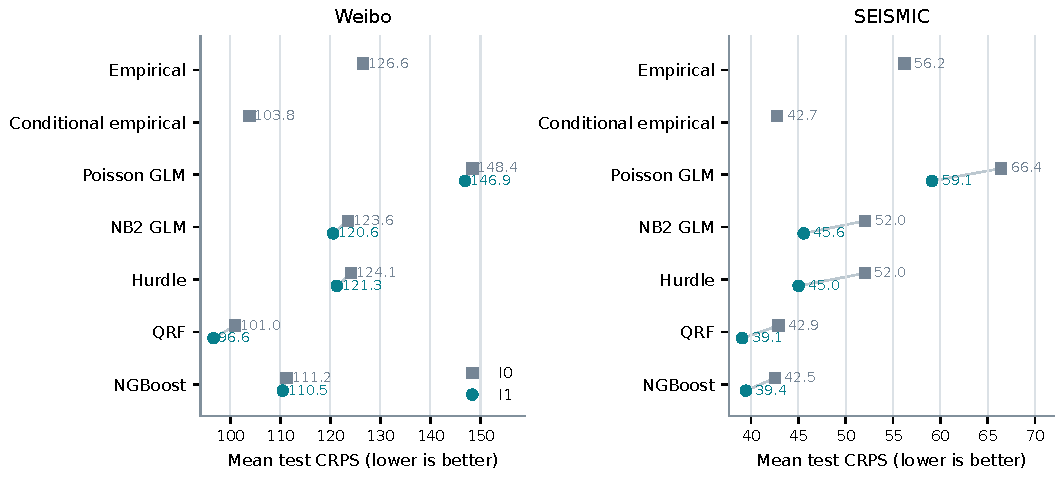
\includegraphics[width=\textwidth]{figures/all_procedures.pdf}
\caption{Descriptive mean CRPS for every complete procedure. Squares denote size and duration ($I_0$); circles add timing ($I_1$). Conditional empirical forecasts establish a strong size-based reference. All comparisons retain the source-specific count units.}\label{fig:all}
\end{figure*}

Ordinary NB2 and Hurdle are close under size-only SEISMIC inputs. On Weibo, NB2 has lower CRPS than Hurdle under both information sets. The zero-handling mechanism therefore does not by itself determine the overall distribution-score ranking.

\hypertarget{distribution-score-gains-coexist-with-calibration-limitations}{%
\subsection{Distribution-score gains coexist with calibration limitations}}

No-growth Brier loss, median absolute error and 90\% interval score all improve descriptively in the six primary information comparisons. Table~\ref{tab:calibration} provides Brier loss and 90\% coverage for these families. Coverage changes have a mixed interpretation. SEISMIC QRF's 90\% coverage rises from 92.42\% to 93.99\%, farther above nominal, even as its interval score improves from 387.892 to 367.088. Its mean width falls from 284.852 to 276.571. The lower proper-score loss captures improvements not summarized by closeness of this single coverage rate to 90\%.


\begin{table*}[t]
\caption{No-growth Brier loss and nominal 90\% coverage. Descriptive secondary results.}\label{tab:calibration}
\centering\footnotesize\setlength{\tabcolsep}{3pt}\renewcommand{\arraystretch}{1.17}
\begin{tabularx}{\textwidth}{>{\hsize=0.72\hsize\linewidth=\hsize\raggedright\arraybackslash}X>{\hsize=0.8400000000000001\hsize\linewidth=\hsize\raggedright\arraybackslash}X>{\hsize=1.02\hsize\linewidth=\hsize\raggedright\arraybackslash}X>{\hsize=1.02\hsize\linewidth=\hsize\raggedright\arraybackslash}X>{\hsize=1.2000000000000002\hsize\linewidth=\hsize\raggedright\arraybackslash}X>{\hsize=1.2000000000000002\hsize\linewidth=\hsize\raggedright\arraybackslash}X}
\toprule
\textbf{Source} & \textbf{Family} & \textbf{Brier I0} & \textbf{Brier I1} & \textbf{Coverage I0} & \textbf{Coverage I1} \\ \midrule
Weibo & Hurdle & 0.016337 & 0.011839 & 94.96\% & 94.99\% \\
Weibo & QRF & 0.015019 & 0.010319 & 91.98\% & 92.58\% \\
Weibo & NGBoost & 0.016345 & 0.015661 & 92.21\% & 92.51\% \\
SEISMIC & Hurdle & 0.007973 & 0.005113 & 94.43\% & 94.13\% \\
SEISMIC & QRF & 0.007908 & 0.005924 & 92.42\% & 93.99\% \\
SEISMIC & NGBoost & 0.007992 & 0.006595 & 93.30\% & 92.41\% \\
\bottomrule\end{tabularx}
\end{table*}


The count PIT panels show substantial nonuniformity for Hurdle, particularly on Weibo, and smaller but persistent departures for the forest and boosting procedures. Timing does not uniformly flatten those distributions. The ordinary Poisson reference illustrates a more severe problem: its timing-augmented nominal 90\% intervals cover only 12.38\% of Weibo cases and 18.63\% of SEISMIC cases. Extra timing predictors do not compensate for this distributional mismatch. Full coverage, interval-score and reliability summaries are retained in the supplement.

\begin{figure*}[t]\centering
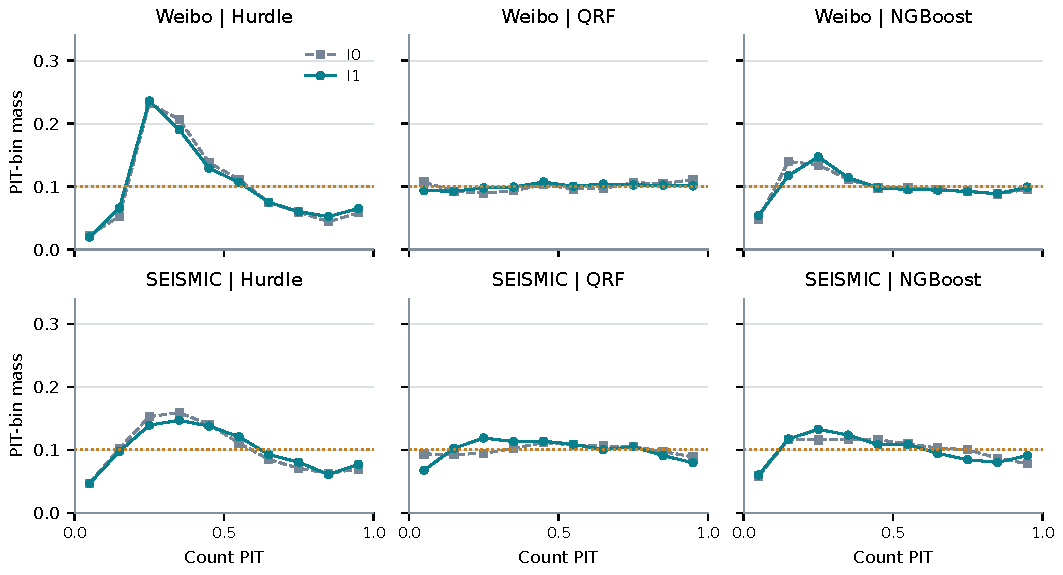
\includegraphics[width=\textwidth]{figures/calibration_overview.pdf}
\caption{Aggregate nonrandomized count PIT-bin mass, averaged across the prescribed seeds and windows. The horizontal dotted line marks 0.1 for ten bins. Both sources use identical vertical axes. The supplement includes all per-window randomized and nonrandomized panels. These are marginal descriptive diagnostics.}\label{fig:calibration}
\end{figure*}

\hypertarget{duplicate-sensitivity-and-completeness}{%
\subsection{Duplicate sensitivity and completeness}}

Three Weibo test roots carry the frozen exact-duplicate-token flag. Removing them only for the planned descriptive sensitivity leaves all three timing contrasts negative: -2.520 for Hurdle, -3.737 for QRF and -0.641 for NGBoost. Absolute score levels change considerably; QRF I0/I1 become 90.725/86.988 compared with 100.990/96.640 on the full sample. A small number of large cases therefore affects the magnitude of aggregate scores. This sensitivity preserves the direction of the descriptive contrasts without establishing unique-event validity or removing possible training effects of duplicate records. SEISMIC's duplicate status remains unknown where event identifiers are unavailable.

All selected primary test procedures are complete. Independent saved-output checks recover the reported aggregates; computational verification is documented in Supplementary Section S6.

\hypertarget{prefix-size-strata-show-heterogeneous-timing-effects}{%
\subsection{Prefix-size strata show heterogeneous timing effects}}

Figure~\ref{fig:strata} shows every source, window and family slot.

\begin{figure*}[t]\centering
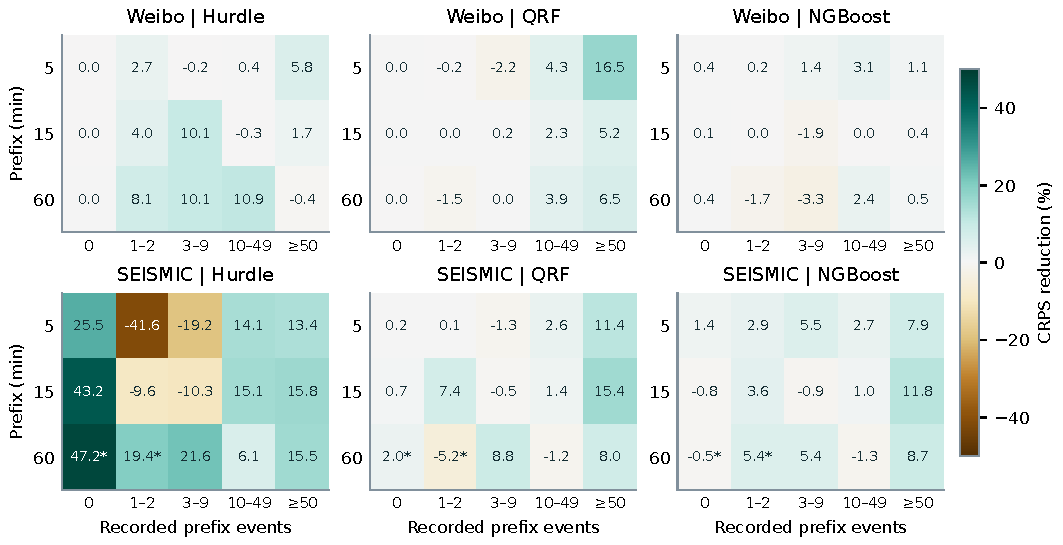
\includegraphics[width=\textwidth]{figures/timing_strata.pdf}
\caption{All 90 supplementary source/family/window/stratum point reductions in CRPS. Positive values favor timing; negative values favor size-only inputs. Color uses one common symmetric scale. Asterisks identify the six point estimates whose exploratory intervals were withheld for fewer than 30 sampling units. Complete pointwise intervals and both empirical references are in the supplement.}\label{fig:strata}
\end{figure*}

The supplementary tables cover all 30 source/window/bin slots and all three primary families. For QRF, the at-least-50-event stratum favors I1 at each window in both sources. Its descriptive relative reductions are 16.50\%, 5.19\% and 6.53\% on Weibo, and 11.38\%, 15.35\% and 8.03\% on SEISMIC at 5, 15 and 60 minutes. Behavior in smaller strata is mixed: SEISMIC QRF at 60 minutes has a 1.21\% increase in CRPS for 10--49 events, while Weibo QRF at five minutes has a 2.20\% increase for 3--9 events. Hurdle and NGBoost display other patterns. These results describe a recurring dense-prefix QRF pattern within the selected archives, not a common curve or a validated threshold across procedures.

Empty prefixes clarify the meaning of the contrast. Their seven timing inputs are the same deterministic defaults within each window. Nevertheless, SEISMIC Hurdle shows a 25.52\% descriptive reduction for its 103 empty five-minute prefixes. The added features cannot convey observed event times within that subgroup. The fitted response at the empty-prefix input has changed through estimation over the full training sample. Thus an I1-I0 subgroup improvement is a property of the fitted procedures and cannot automatically be assigned to locally observed timing information.

At 60 minutes, SEISMIC has only 26 empty-prefix roots and 20 roots with 1--2 events; their point estimates are retained and intervals are withheld under the specified rule. All other slot counts, both empirical references, family results and pointwise intervals are available in Supplementary Section S8 and the machine-readable tables.

\hypertarget{timing-retains-its-advantage-over-the-independent-noise-control}{%
\subsection{Timing retains its advantage over the independent-noise control}}

\begin{figure*}[t]\centering
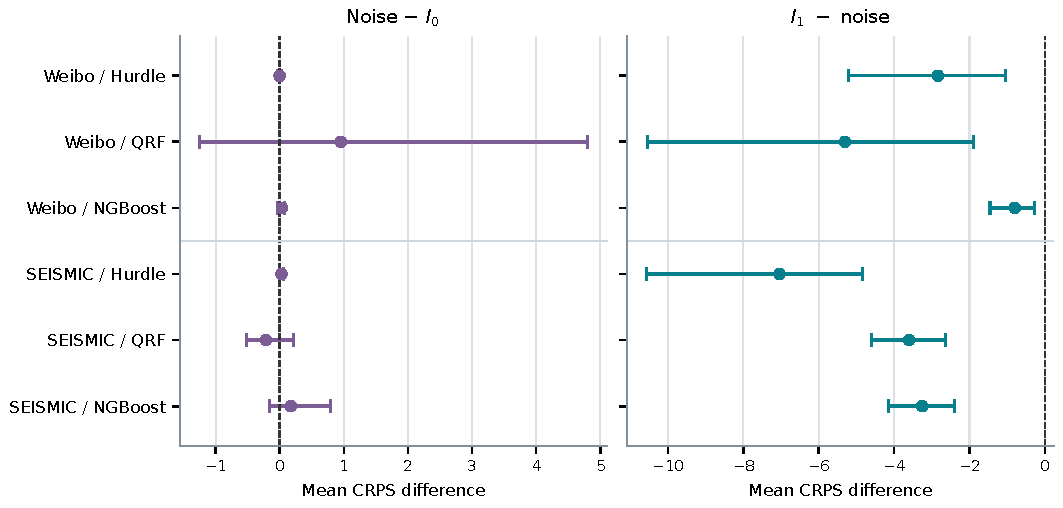
\includegraphics[width=\textwidth]{figures/noise_control.pdf}
\caption{All 12 supplementary negative-control contrasts with separately Bonferroni-adjusted conditional intervals. Noise minus $I_0$ has mixed point signs and intervals spanning zero; this does not establish equivalence. Every $I_1$ minus noise interval lies below zero. Noise losses average the three fixed noise realizations and the prescribed fitting seeds.}\label{fig:noise}
\end{figure*}

Table~\ref{tab:noise} reports all supplementary control contrasts. Noise-I0 point estimates are mixed and every adjusted interval includes zero. Timing has lower CRPS than the noise control in all six cases, with adjusted intervals entirely below zero. Relative reductions against noise range from 0.72\% to 5.20\% on Weibo and from 7.63\% to 13.52\% on SEISMIC. These are point summaries of the averaged control procedure.


\begin{table*}[t]
\caption{Supplementary dimension-matched noise control. Intervals use a separate family of 12 Bonferroni-adjusted contrasts.}\label{tab:noise}
\centering\footnotesize\setlength{\tabcolsep}{3pt}\renewcommand{\arraystretch}{1.17}
\begin{tabularx}{\textwidth}{>{\hsize=0.5\hsize\linewidth=\hsize\raggedright\arraybackslash}X>{\hsize=0.6\hsize\linewidth=\hsize\raggedright\arraybackslash}X>{\hsize=0.65\hsize\linewidth=\hsize\raggedright\arraybackslash}X>{\hsize=1.625\hsize\linewidth=\hsize\raggedright\arraybackslash}X>{\hsize=1.625\hsize\linewidth=\hsize\raggedright\arraybackslash}X}
\toprule
\textbf{Source} & \textbf{Family} & \textbf{Noise CRPS} & \textbf{Noise - I0 {[}adjusted interval{]}} & \textbf{I1 - noise {[}adjusted interval{]}} \\ \midrule
Weibo & Hurdle & 124.124 & -0.002 {[}-0.036, +0.030{]} & -2.838 {[}-5.212, -1.050{]} \\
Weibo & QRF & 101.944 & +0.953 {[}-1.255, +4.803{]} & -5.304 {[}-10.532, -1.905{]} \\
Weibo & NGBoost & 111.283 & +0.033 {[}-0.036, +0.080{]} & -0.799 {[}-1.457, -0.274{]} \\
SEISMIC & Hurdle & 52.063 & +0.027 {[}-0.002, +0.056{]} & -7.041 {[}-10.573, -4.833{]} \\
SEISMIC & QRF & 42.660 & -0.216 {[}-0.515, +0.212{]} & -3.602 {[}-4.594, -2.648{]} \\
SEISMIC & NGBoost & 42.697 & +0.174 {[}-0.160, +0.793{]} & -3.257 {[}-4.145, -2.392{]} \\
\bottomrule\end{tabularx}
\end{table*}


The timing advantage therefore persists against this specified uninformative augmentation. The intervals containing zero do not establish equivalence between noise and I0, and the control does not equate effective capacity. For example, the Weibo QRF noise-I0 interval spans -1.255 to +4.803 CRPS units; meaningful changes in either direction remain compatible with that interval. Separate realization summaries, including favorable noise outcomes, are retained in Supplementary Section S8. All scheduled control procedures and test scores completed. {\small\textit{Preparation:~\cite{openai2026}.}}
